\documentclass[10pt,twocolumn]{article} 

% use the oxycomps style file
\usepackage{oxycomps}

% read references.bib for the bibtex data
\bibliography{references}

% include metadata in the generated pdf file
\pdfinfo{
    /Title (Ethics Paper)
    /Author (Sammy Sanchez)
}

% set the title and author information
\title{CS Ethics Paper about My COMPS Project}
\author{Sammy Sanchez}
\affiliation{Occidental College}
\email{sanchezs@oxy.edu}

\begin{document}

\maketitle

\begin{abstract}

 In this paper I will discuss the ethics against how statistical data is gathered and how the data can be manipulated against certain basketball players. Data bias is a huge reason people argue that one player is better than other and how my project might strengthen those views. Even though the data is accessible to everybody that looks it up, certain aspects of the stats can be used to give a negative view towards players based on the stats used. I will also discuss how technology might not help solve this problem of picking a better player with data visualization because of how you would need to watch basketball games to decide the impact. These ethical concerns can be a big problem because of the power of how someone can used the data for thinking other players are worse than others and can spread that information over the internet like Twitter causing negativity towards that player. It will hard addressing all the ethical concerns behind my project because of how people will analyze the data for themselves to determine who they want to pick and that could include their own personal biases like favorite team or likeness of the player. 
    

\end{abstract}

\section{Data Bias}

Data bias in basketball stats can be an ethical problem because of what stats the person chooses to evaluate a player or players and contributes to the person thinking that they are not valuable. There are always arguments of what specific stats are more valuable compared to other stats. If a person using my project wanted to see if one player is better than another player using a specific stat and seeing the visualization on a graph, it can influence their decision and lets the users assume that one is better than the other which can lead to the NBA player being scrutinized online.  

An example of data bias that would be used in my project would be the discussion of the 2022 NBA MVP award. In recent NBA news when discussing who the MVP of the season should be, the players are compared using Advanced Statistics and point to Nikola Jokic to win the award. The advanced stats used were RAPTOR, EPM, BPM, and LEBRON and showed a chart of the rankings of Nikola Jokic, Giannis Antetokounmpo, Joel Embiid and Devin Booker for these stats. Jokic placed 1st in the advanced stats out of all the MVP candidate players stated above from the article. This is an example of data bias because of how the chosen stats can boost an opinion about one player which makes them seem better than others. The picked stats used to support that opinion of the MVP in the news article were advanced stats and in my project, the same can happen when evaluating a player to use for fantasy sports because of the user chosen stats to analyze. Figure 1 shows how the MVP discussion is influenced by specific stats. 

\begin{figure}
    \centering
    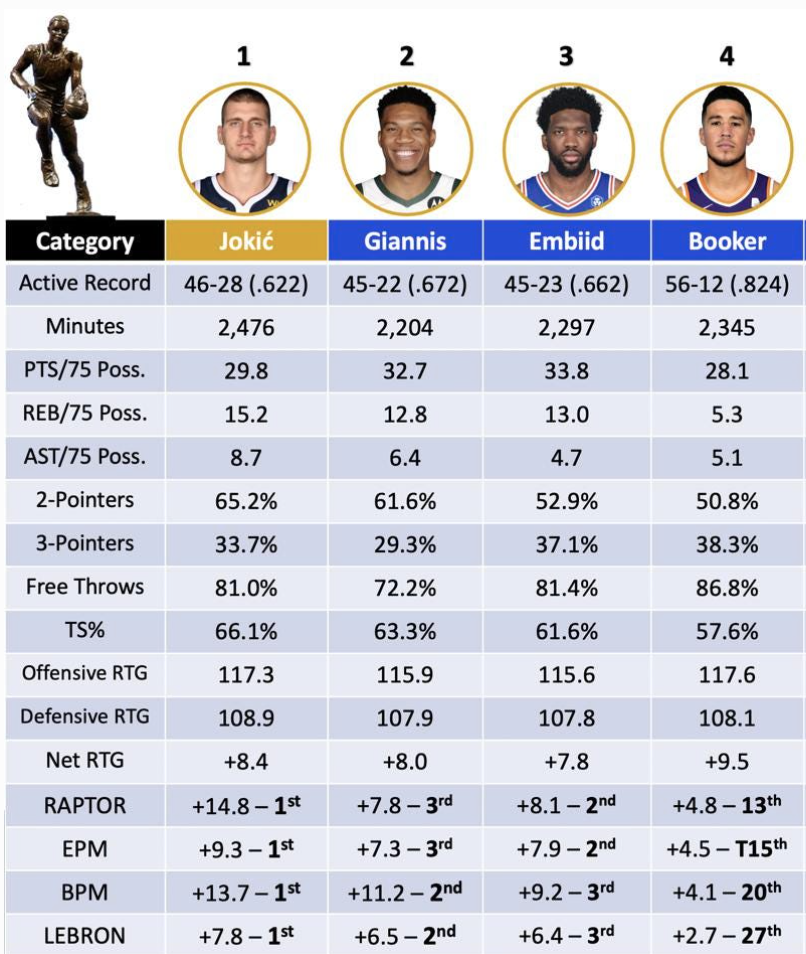
\includegraphics[width=.95\linewidth]{mvp.png}
    \caption{
        The MVP Chart
    }
    \label{fig:first-page}
\end{figure}

The data bias that can come with my project would not be ethical because of how it influences people to think that specific stats are better than other stats. It can lead to NBA players being bashed or hated on for having poor stats for the opinionated "more valuable" stats. Another issue with the data bias problem is that it can affect how other people view specific stats and leads to the potential users of my project to use the stats to support their own biases about a player because of how well they rank in the "more valuable" stats. The article I referenced is written by Forbes writer \textcite{MVPJokic}.

\section{Technological Solutionism}

For technological solutionism, sometime when evaluating stats and a player, it comes down to watching the NBA games because technology cannot predict everything accurately. When using my project to evaluate players, it potentially will not be the best solution because of how players play differently in game situations and that there are not stats that are measured to add value to a player. My project would not be ethical because of how it will not account for the variables that happen in a NBA game that do not show up on a stat sheet or are not measured. 

An example of how technology is not always the answer would be how NBA players have an impact in the basketball game when their stats are not considered better than another player. In an article written about players who are worth more than their stats, it discusses five different players and their impact on the court which is a variety of factors not truly measured by stats. The players are Draymond Green, Jimmy Butler, Marcus Smart, Jrue Holiday, and Mikal Bridges and each one does something that is not measured on the box score. Bridges hits open shots at a high rate because of how his teammates get doubled teamed. Green plays defense against any position in the NBA which is hard for his size at 6'6" and can be a playmaker like a guard. Butler has a strong mentality and leadership which allows his team to flourish better with him on the court. Smart plays great defense being a point guard and can hit 3's and be a playmaker which brings value to his team. Holiday can make clutch plays and hit clutch shots. All of these factors I mentioned are based on people watching the basketball games with these players playing. The article I used was written by \textcite{NoStatSheet}. In Figure 2, Draymond Green's team does worse without him and play better with him and it is not a stat that is measured for value on sport database websites.

\begin{figure}
    \centering
    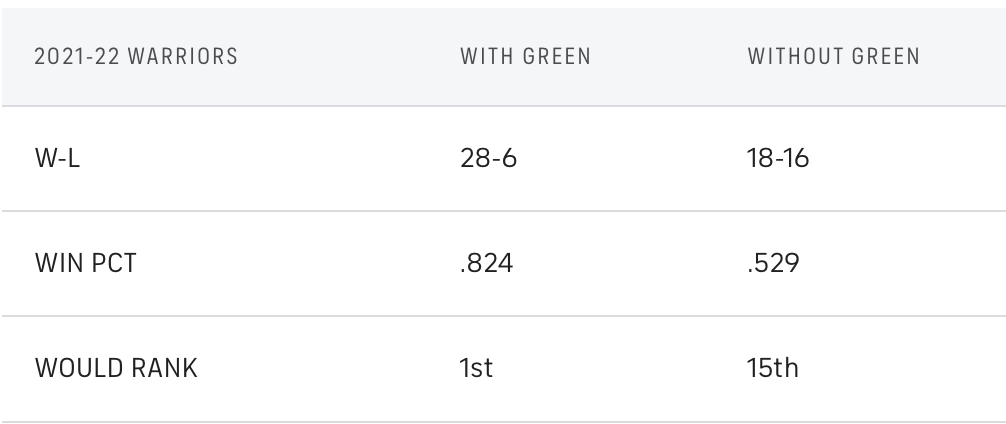
\includegraphics[width=.95\linewidth]{Green_stats.png}
    \caption{
       Non-measured Draymond Green Stats from 2021-22 Season
    }
    \label{fig:second-page}
\end{figure}

In my project, it will not factor in these examples of player's values when doing a stats visualization and can be not ethical because of how it will ignore these factors. It questions if a player's value is only measured by statistical data and my project cannot watch a game to see those non-measured values. My project would not be ethical because of how it does not include the non-statistical value and would not be fair to evaluate the player based on only stats when doing the data visualization. Technology is sometimes not needed for determining value of a player because of how impact of certain attributes of a NBA game is not measured and would not be fair to purposely use my project to find out what player is better other than using statistics. 

\section{Personal Bias}

\begin{figure}
    \centering
    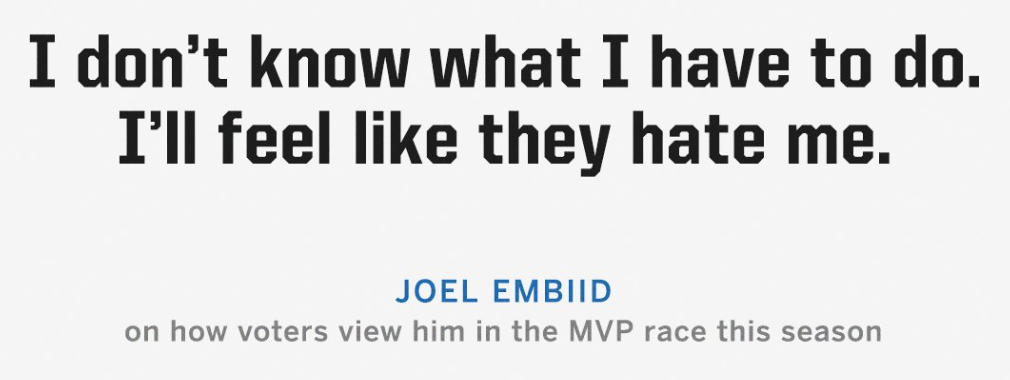
\includegraphics[width=.95\linewidth]{Joel_quote.png}
    \caption{
       Joel Embiid Quote About Being MVP
    }
    \label{fig:second-page}
\end{figure}
Personal bias can also be a factor of why my project would not be ethical. The bias comes with being a fan of basketball and people like certain players and dislike certain players because of various reasons. Some reasons could be location biased and you are a fan of the team the player plays for or you can hate a player because of their demeanor (ex: yelling a lot during the game, the player saying something you did not agree with when being interviewed, etc.) The personal bias could affect how my project is used because if someone were to compare a player to other players and they see that one player they do not like is closely similar statistically, it may leave them to pick someone else for their fantasy team and that the user evaluation was based on personal biases. 

In an article written about Joel Embiid who is a MVP candidate, it talks about how the media dictates who wins the awards and how they might not pick him because of personal biases against him. This would relate to what I am discussing because of how a personal bias can determine evaluation and how the person could ignore statistical data of the player. Figure 3 shows a quote of Embiid talking about the media voters not liking him so it makes him think he will not win the MVP based on being disliked which is a personal bias. In the article written by Prince \textcite{MVPBias}, he mentions all the stats that can point to Embiid winning the MVP and the problems with the media picking the MVP because it differentiates every season with a different narrative. Personal bias drive the conversation on who wins MVP and it sometimes is not all about statistical data which can relate to my COMPS project.

When using my project for evaluating NBA players to choose, there can be personal biases against certain players because the users can dislike a person for various reasons. That influences how a user would choose a player and can lead to narratives that a player is negative because of those views like displayed in the media. It would not be fair to the player to be ignored when statistical data can back up that player to be impactful on a fantasy team. People have their own opinions on how a player should be evaluated but overall it can be in a non ethical way when using personal biases.


\printbibliography 

\end{document}
